\section{Aluminiumoxid-ALD}
\label{aluminaald}

Einen Vorzeige-Prozess für Atomlagenabscheidungen bildet die Abscheidung von Aluminiumoxid \ce{Al2O3}\cite{puurunen_surface_2005}, für die häufig das Precursorpaar Trimethylaluminium (TMA, \ce{Al(CH4)3}) und Wasser genutzt wird.
Aufgrund seiner relativ hohen Permittivität von $k\approx 8$ ersetzt \ce{Al2O3} langsam gemeinsam mit Materialien wie \ce{HfO2} und \ce{ZrO2}, welche ebenfalls per Gasphasenabscheidung produziert werden können\cite{smith_chemical_2000}, Siliziumdioxid ($k=3.9$) als Dielektrikum in der Halbleiterindustrie.
Deshalb soll der TMA-\ce{H2O}-Prozess im Folgenden besonders hinsichtlich der Reaktion der Precursormoleküle mit der Oberfläche untersucht werden.

Dazu wurden verschiedene Parametersätze hinsichtlich der Anwendbarkeit auf reaktive Oberflächenabscheidungen untersucht, und schließlich erste Oberflächenreaktionen mit ihnen simuliert.
Dabei ist bisher lediglich die Simulation der reaktiven Hydroxylierung der Oberfläche gelungen, was auf die mangelhafte Beschreibung der \ce{Al-C}-Bindungen mit den benutzten Potentialen zurück zu führen ist.

\subsection{Parametersätze}

Für die MD-Simulation von \ce{Al2O3} stehen drei Parametrisierungen zur Verfügung, die bereits aus den Untersuchungen der Silizium-Potentiale bekannt sind (Abschnitt~\ref{siliconpvd}):\\
\pot{Al\_AlO\_AlN} aus LAMMPS\cite{plimpton_lammps_2014}, \pot{liu\_ettringite}\cite{liu_development_2012}, welches nachfolgend nur als \pot{liu} geführt werden soll, und \pot{narayanan}\cite{narayanan_reactive_2012}.
Ihnen ist gemein, dass sie ausgehend von Silizium-Parametrisierungen um Parameter für Aluminium-Verbindungen erweitert wurden, weshalb sie auch im vorherigen Kapitel untersucht wurden.
Auf eine Bewahrung der Konsistenz der Siliziumparameter wurde dabei scheinbar verzichtet, so dass etwa mit der \pot{liu}-Parametrisierung eine verlässliche Simulation von Silizium-Verbindungen verhindert, im Gegenzug aber die Simulation von Aluminium-Verbindungen ermöglicht wird.
Eine Kombination verschiedener Parametrisierungen ist zwar denkbar und wird bereits kommerzieller Software durchgeführt\cite{biovia_materials_2014}, würde aber für die vorliegenden Potentiale höchstens zweifelhafte Verbesserungen bringen.

Die \pot{Al\_AlO\_AlN}-Datei stammt direkt aus der offiziellen LAMMPS-Distribution\cite{plimpton_lammps_2014}, wurde jedoch am 17. Mai 2013 während der Ergänzung von Referenzen auf wissenschaftliche Publikationen in anderen Parameterdateien kommentarlos aus dem Paket entfernt\cite{thompson_lammps_2013}.
Bei den Recherchen konnte kein Hinweis auf das ursprüngliche Anwendungsgebiet gefunden werden, weshalb mit diesen Parametern berechnete Eigenschaften mit Vorsicht überprüft werden.

Das \pot{liu}-Potentialdatei wurde für die Simulation von Ettringit (\ce{Ca6[Al(OH)6]2(SO4)3 26H2O}) erstellt, welches \ce{Al-O}-Bindungen und \ce{OH}-Gruppen enthält, sodass zumindest die Simulation des Bulkmaterials und einer hydroxylierten Oberfläche aussichtsreich erscheint.
Sie beschreibt die Oberflächenhydroxylierung und stellt sich daher als Favorit für Parsivald-Simulationen heraus, obwohl ihr eigentliches Anwendungsgebiet auf der Simulation von Kristallen liegt.

Zuletzt steht die \pot{narayanan}-Parametrisierung für \ce{Li-Al}-Silikate, insbesondere zur Simulation von Eukryptit (\ce{LiAl[SiO4]}), zur Verfügung, lässt aber keine endgültige Aussage über die Qualität der \ce{Al-O}-Bindungen und \ce{OH}-Gruppen zu.
Zwar besteht ihr Trainingssatz aus verschiedenen Lithium-Aluminium-Kristallen, aber nur $\gamma$-\ce{LiAlO2} beinhaltet direkte \ce{Al-O}-Bindungen, wo hingegen keine der Strukturen Hydroxylgruppen beinhaltet.
Es ist daher unwahrscheinlich, dass die \pot{narayanan}-Potentialdatei komplizierte Systeme verlässlich darstellt.

\subsection{Voruntersuchungen}

Wie in den vorherigen Abschnitten werden hier separate Voruntersuchungen durchgeführt, zu denen die Reaktion von Precursormolekülen mit der Oberfläche ergänzt wurde.
Die Referenzwerte sind in Anhang~\ref{appendix_constants} zusammen gefasst.

\subsubsection{Vergleich der strukturellen Eigenschaften von \ce{Al2O3}}

Zum Vergleich der strukturellen Eigenschaften des Bulkmaterials wurde in MD-Simulationen ein $\alpha$-\ce{Al2O3}-Kristall bei \SI{1500}{\kelvin} für \num{100000} Zeitschritte isotherm-isobar relaxiert und vor den abschließenden Messungen auf Raumtemperatur herunter gekühlt.
Die Abkühlung wurden versehentlich um einen Faktor 10 zu schnell durchgeführt, weshalb die beobachteten Dichten vorsichtig mit experimentellen Werten zu vergleichen sind, da sie noch vom Wert bei höheren Temperaturen dominiert sein können.
Eine erneute Berechnung der Werte steht noch aus, doch zeigen sich anhand der Dichten der amorpher Strukturen genügend Hinweise auf die Anwendbarkeit der Parametrisierungen.
Referenzwerte der Dichten für unterschiedliche Temperaturen liegen bei \SI{3.99}{\gpcc} bei Raumtemperatur und \SI{3.80}{\gpcc} bei \SI{1500}{\kelvin}\cite{fiquet_high-temperature_1999}.
Bindungslängen und Koordinationszahlen wurden direkt aus der RDF kristalliner Strukturen bestimmt.
Ihre Referenzwerte wurden auf die gleiche Weise durch die Untersuchung der idealen Kristallstruktur bestimmt, welche mittels Materials Studio\cite{biovia_materials_2014} auf Basis eines $\alpha$-\ce{Al2O3}-Kristalles präpariert wurde.
Aufgrund identischer Dichten und übereinstimmender Kristallgitter\cite{haynes_crc_2011} ist dabei von einer guten Übereinstimmung der Referenzwerte mit experimentellen Werten auszugehen.

Für die Bestimmung der Dichte der amorphen Struktur wurde das Bulkmaterial über den Schmelzpunkt von \SI{2317}{\kelvin} auf \SI{2555}{\kelvin} erhitzt, auf dieser Temperatur relaxiert und langsam auf Raumtemperatur abgekühlt.
Aufgrund der strukturellen Vielfalt bei amorphen Aluminiumoxiden liegt der Referenzbereich der Dichte von gasphasen-abgeschiedenen \ce{Al2O3}-Schichten zwischen \SI{3.2}{\gpcc} und \SI{3.9}{\gpcc}\cite{wang_dependence_1997}.

\begin{table}[b!]
  \oddrowcolors
  \caption[Vergleich struktureller Eigenschaften von $\alpha$-\ce{Al2O3}]{
    Vergleich struktureller Eigenschaften von \ce{Al2O3} für verfügbare ReaxFF-Parametrisierungen.
    Referenzwerte stammen von einer relaxierten Kristallstruktur.
  }
  \label{tab:aluminabulks}

  \begin{tabularx}{\textwidth}{|Xllll|}
    \hline
    \textbf{\pot{Eigenschaft}}          & \textbf{\pot{Referenz}} & \textbf{\pot{Al\_AlO\_AlN}} & \textbf{liu}         & \textbf{narayanan}   \\
    \hline
    Dichte, $\alpha$-kristallin         & \SI{3.98}{\gpcc}        & \SI{4.31}{\gpcc}            & \SI{3.88}{\gpcc}     & \SI{3.76}{\gpcc}     \\
    Dichte, amorph                      & \SI{>3.2}{\gpcc}        & ~                           & \SI{3.66}{\gpcc}     & \SI{2.93}{\gpcc}     \\
    \ce{Al-O}-Bindungslänge, kristallin & \SI{1.90}{\angstrom}    & \SI{1.94}{\angstrom}        & \SI{1.88}{\angstrom} & \SI{1.85}{\angstrom} \\
    \ce{Al-O}-Koordination, kristallin  & \num{4.00}              & \num{5.40}                  & \num{4.55}           & \num{4.05}           \\
    \ce{Al-Al}-Koordination, kristallin & \num{4.00}              & \num{6.66}                  & \num{5.98}           & \num{5.10}           \\
    \ce{O-O}-Koordination, kristallin   & \num{12.0}              & \num{12.4}                  & \num{11.0}           & \num{12.2}           \\
    \hline
  \end{tabularx}
\end{table}

Die Verteilung der Koordinationszahlen amorpher Schichten wurde in dieser Arbeit nicht näher untersucht, da einerseits nur Vergleiche mit anderen MD-Rechnungen zur Verfügung stehen\cite{gutierrez_molecular_2002}, andererseits ein eigenes Werkzeug hätte geschrieben werden müssen.
Eine Integration eines solchen Werkzeuges zur Bestimmung der Verteilung der Koordinationen in Parsivald könnte allerdings helfen, die Struktur der Schicht während der laufenden Simulation zu untersuchen.

Die Ergebnisse dieser Untersuchungen (Tabelle~\ref{tab:aluminabulks}) zeichnen ein vielseitiges Bild.
Einerseits stimmt die kristalline Bindungslänge für alle Parametrisierungen auf weniger als \SI{3}{\percent} überein, andererseits ergeben sich große Unterschiede in der Dichte der Kristalle, die mit einer leichten Verformung der Kristallstrukturen einher geht und dabei nicht mit den Bindungslängen korreliert ist.
Im Fall von \pot{Al\_AlO\_AlN} weicht die kristalline Dichte um \SI{+8.3}{\percent} ab und übersteigt die Dichte der dichtesten \ce{Al2O3}-Kristalle bei Normaldruck, was sich auch an den überschätzten Koordinationszahlen zeigt.
Die beiden verbleibenden Parametersätze zeigen eine geringere Dichte, die sich der von $\gamma$-\ce{Al2O3} mit \SI{3.67}{\gpcc}\cite{dynys_alpha_1982} nähert.

Eine Bestimmung der amorphen Dichten für die \pot{liu}- und \pot{narayanan}-Parametersätze zeigt für \pot{liu} mit \SI{3.66}{\gpcc} eine amorphe Dichte im erwarteten Bereich, während \pot{narayanan} bei allen Simulationen eine Dichte von \SI{2.93}{\gpcc} erreicht und damit unterhalb der beobachteten Werte liegt, obwohl es die besten Ergebnisse für kristalline Strukturen zeigt.

\subsubsection{Simulationen der Stabilität von Precursormolekülen}

Die Stabilität für Trimethylaluminium (TMA) wurde nach dessen manueller Präparation für die drei Parametersätze \pot{Al\_Al0\_AlN}, \pot{liu\_ettringite} (kurz \pot{liu}) und \pot{narayanan} untersucht (Abbildung~\ref{fig:tmastability}).
Die genutzten Strukturdaten\cite{haynes_crc_2011} sind in Anhang~\ref{appendix_constants} zusammen gefasst.

Mit den \pot{Al\_Al0\_AlN}-Parametern konnte TMA stabil simuliert werden (Abbildung~\ref{fig:tmamonomer}), jedoch nehmen die simulierten Moleküle keine planare Struktur ein, sondern weisen reduzierte \ce{C-Al-C}-Bindungs\-winkel von durchschnittlich \SI{103}{\degree} auf, wodurch sich eine angewinkelte Struktur ergibt.
Die Bindungslängen stimmen hingegen mit durchschnittlich \SI{2.020}{\angstrom} (Referenz: \SI{1.957}{\angstrom}\cite{haynes_crc_2011}) für \ce{Al-C} und \SI{1.106}{\angstrom} (Referenz: \SI{1.113}{\angstrom}\cite{haynes_crc_2011}) für \ce{C-H} bis auf \SI{3}{\percent} mit Referenzwerten überein.
Mit dieser Parametrisierung kann ebenfalls das TMA-Dimer bei niedrigen Temperaturen simuliert werden (Abbildung~\ref{fig:tmadimer}).

\begin{figure}[b!]
  \captionsetup[subfigure]{singlelinecheck=false}
  \begin{subfigure}[t]{4cm}
    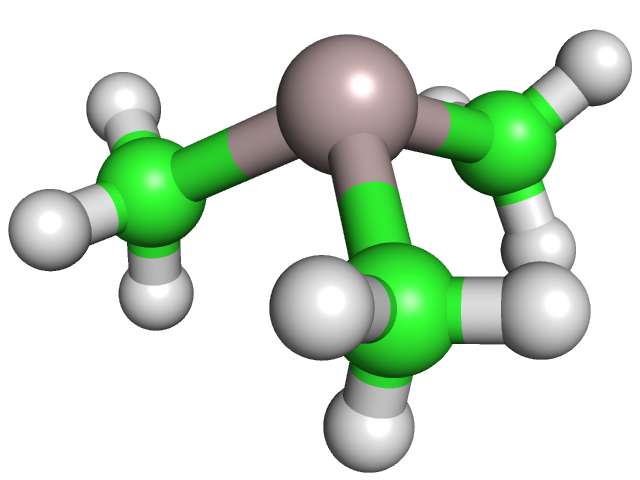
\includegraphics[width=\textwidth]{tma_Al}
    \subcaption{
      \pot{Al\_Al0\_AlN}: \\
      stabiles TMA
    }
    \label{fig:tmamonomer}
  \end{subfigure}
  \hfill
  \begin{subfigure}[t]{5.5cm}
    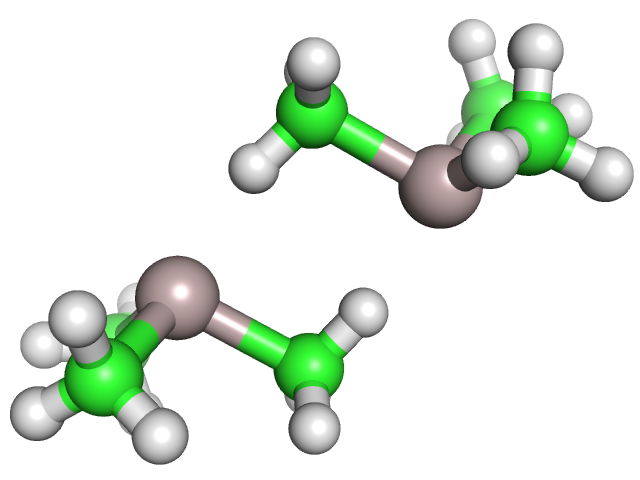
\includegraphics[width=\textwidth]{tma_Al_dimer}
    \subcaption{
      \pot{Al\_Al0\_AlN}: \\
      stabiles TMA-Dimer
    }
    \label{fig:tmadimer}
  \end{subfigure}
  \hfill
  \begin{subfigure}[t]{4.5cm}
    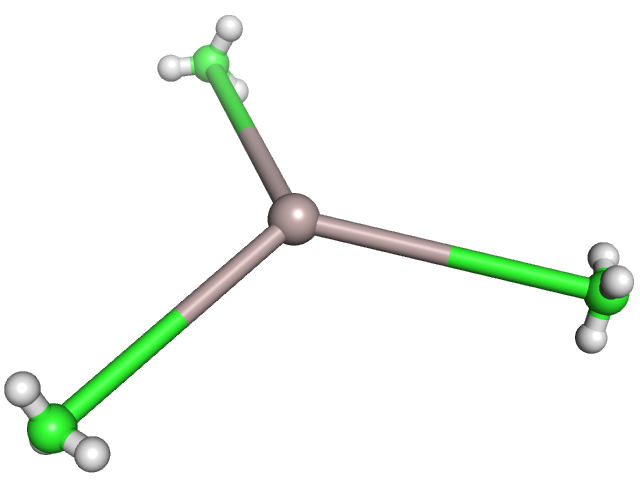
\includegraphics[width=\textwidth]{tma_liu}
    \subcaption{
      \pot{liu\_ettringite}: \\
      Keine \ce{Al-C}-Bindungen
    }
    \label{fig:tmaliu}
  \end{subfigure}

  \caption{Stabilität der TMA-Moleküle für verschiedene \ce{Al2O3}-Parametersätze}
  \label{fig:tmastability}
\end{figure}

TMA-Simulationen mit dem \pot{liu}-Parametersatz zeigen hingegen keinen Erfolg, da er keine \ce{Al-C}-Bindungen beschreibt.
Somit driften in den Simulationen ungebundene Methylgruppen vom zentralen Aluminium-Atom davon (Abbildung~\ref{fig:tmaliu}).
Die \pot{narayanan}-Parametrisierung verfügt über keine Kohlenstoff-Parameter und kann deshalb nicht für TMA-Simulationen genutzt werden.

Simulationen von Wassermolekülen waren hingegen mit allen Parametrisierungen erfolgreich.

Anhand des \pot{Al\_AlO\_AlN}-Parametersatzes wurden auch Simulationen der Reaktionen zwischen TMA und Wasser in der Gasphase versucht, wie sie beispielsweise bei Vermischung der Precursorgase im ALD-Reaktor auftreten können.
Diese zeigten keinen Erfolg, da die \ce{Al-C}-Bindungen in der \pot{Al\_AlO\_AlN}-Parametrisierung entweder zu stark sind oder in zu großem Maß von den Methylgruppen abgeschirmt werden.

\subsubsection{Simulation der Hydroxylierung einer $\alpha$-\ce{Al2O3}-Oberfläche}

Abschließend soll die reaktive Hydroxylierung einer Kristall-Oberfläche mit Wassermolekülen simuliert werden.
Dazu wurde eine Kristalloberfläche mit einer variablen Menge von Wassermolekülen in einem vertikalen Abstand, welcher mit \SI{10}{\angstrom} größer als die ReaxFF-Inter\-aktions\-reich\-weite von \SI{6}{\angstrom}, vorbereitet (Abbildung~\ref{fig:wateraluminasurface-a}) und in einer reinen MD-Simulation mit LAMMPS simuliert.
In der Simulation werden die Wassermoleküle mit einer entsprechend der Maxwell-Distribution bei \SI{500}{\kelvin} versehen, die Atome an der Unterseite des Substrates fest gehalten und das aus Notwendigkeit verwendete Berendsen-Thermostat nur auf den mittleren Teil des Substrates angewandt, um seinen Einfluss auf die Reaktionen zu verringern.
Dabei wird eine chemische Adsorption der Wassermoleküle erwartet\cite{shapovalov_ab_2000}, die zu einer Sättigung der Oberfläche mit Hydroxyl-Gruppen bei einer Bedeckung von \SI{9.2}{\per\square\nano\meter}\cite{kim_energy_2011} führen sollte.
Die Zahl der Wassermoleküle in der Simulation kann in den drei untersuchten Systemen zu Hydroxyl-Bedeckungen von \SI{5.8}{\per\square\nano\meter}, \SI{19.0}{\per\square\nano\meter} und \SI{57.6}{\per\square\nano\meter} führen.

\begin{figure}
  \captionsetup[subfigure]{singlelinecheck=false}
  \def\subfigwidth{0.32\textwidth}
  \begin{subfigure}[t]{\subfigwidth}
    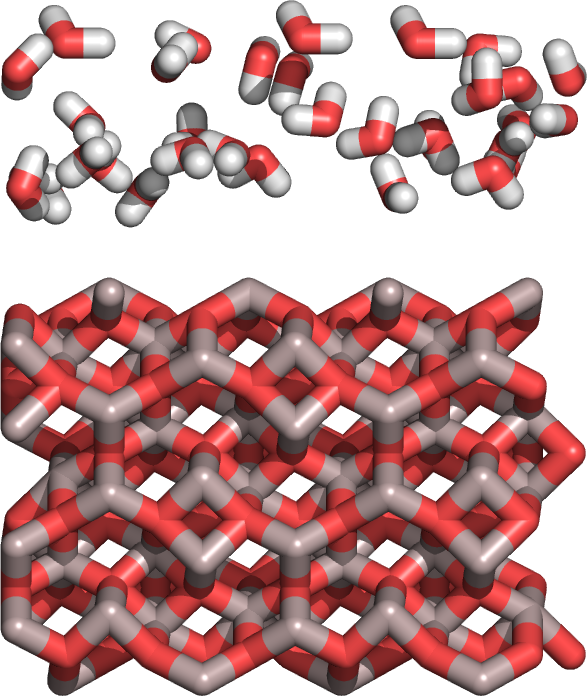
\includegraphics[width=\textwidth]{alumina_h2o_before}
    \subcaption{Seitenansicht, vor der Reaktion}
    \label{fig:wateraluminasurface-a}
  \end{subfigure}
  \hfill
  \begin{subfigure}[t]{\subfigwidth}
    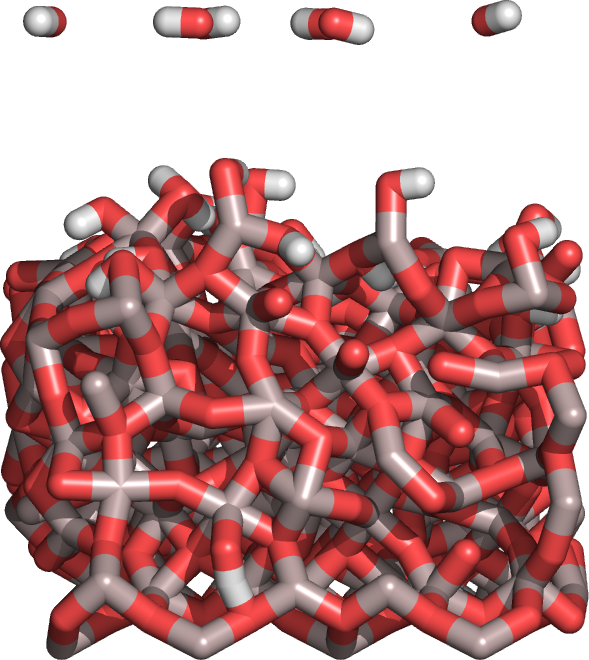
\includegraphics[width=\textwidth]{alumina_h2o_after}
    \subcaption{Seitenansicht, nach der Reaktion}
    \label{fig:wateraluminasurface-b}
  \end{subfigure}
  \hfill
  \begin{subfigure}[t]{\subfigwidth}
    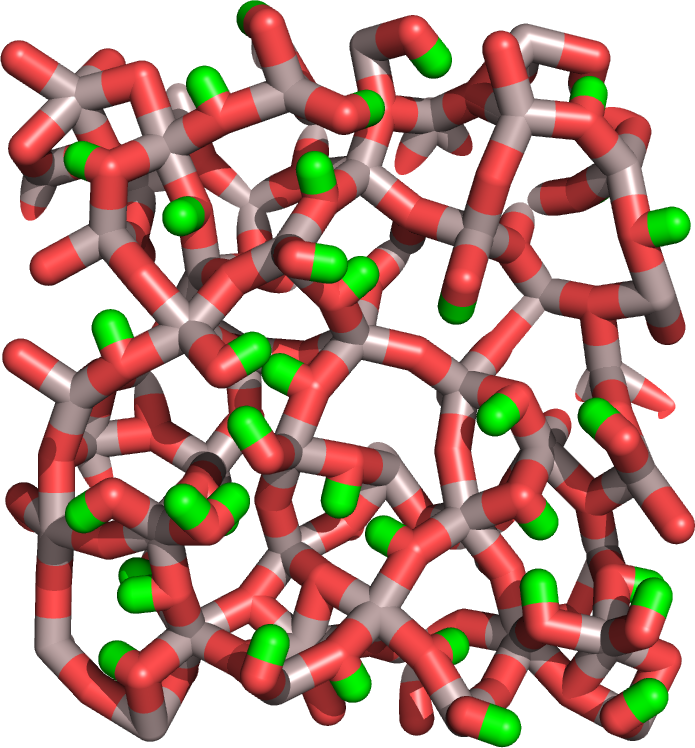
\includegraphics[width=\textwidth]{alumina_h2o_topview}
    \subcaption{Draufsicht, nach der Reaktion.
      \textbf{Hydroxyl} ist grün hervorgehoben.
    }
    \label{fig:wateraluminasurface-c}
  \end{subfigure}
  \caption[Oberflächenreaktion von Wasser mit $\alpha$-\ce{Al2O3}]{Ergebnisse einer Oberflächenreaktion von Wasser mit $\alpha$-\ce{Al2O3}.
    Das Wasser reagiert mit Sauerstoffatomen an der Oberfläche zu Hydroxylgruppen.
  }
  \label{fig:wateraluminasurface}
\end{figure}

Mit den \pot{narayanan}-Parametern konnten keine Adsorptionen beobachtet werden, da sie in den Simulationen durch eine repulsive Kraft zwischen den Wassermolekülen und der Oberfläche verhindert werden.
Das deutet darauf hin, dass Hydroxylgruppen auf einer Aluminiumoxid-Oberfläche von dem Parametersatz energetisch nicht bevorzugt werden oder die Reaktion mit einer übermäßig hohen Reaktionsbarriere verbunden ist.
Zusammen mit dem Problem, Trimethylaluminium nicht darstellen zu können, ist dieser Parametersatz somit nicht in der Lage, den ALD-Prozess durch seine Precursor-Oberflächen-Reaktionen zu beschreiben.

Das Ergebnis der Simulationen für die \pot{liu}-Parameter (Abbildungen~\ref{fig:wateraluminasurface-b} und~\ref{fig:wateraluminasurface-c}) zeigt jedoch die gleichmäßige Bedeckung der Oberfläche mit Hydroxylgruppen (\SI{9.5}{\per\square\nano\meter}) neben gelegentlich adsorbierten Wassermolekülen, die keine Oberflächenreaktion eingegangen sind.
Letztere sollten sich aber auf längere Sicht durch die Einflüsse der Überkoordinationsterme des ReaxFF-Potentiales von der Oberfläche lösen oder eine Reaktion mit benachbarten Sauerstoff-Atomen eingehen.
Trotz der unterschiedlichen Startbedingungen stimmt der Bedeckungsgrad der Oberfläche mit Hydroxylgruppen den Maximalwerten von \SI{9.2}{\per\square\nano\meter}\cite{kim_energy_2011} überein.
Die verbleibenden Wassermoleküle sind keine Adsorption auf der Oberfläche eingegangen sondern in der Gasphase verblieben, wie in Abbildung~\ref{fig:wateraluminasurface-b} am oberen Rand des periodischen Simulationsraumes erkennbar ist, bei denen sie durch periodische Randbedingungen zerteilt erscheinen.
Es konnte damit gezeigt werden, dass die Begrenzung der Reaktion von Wasser durch die sterische Hinderung der Wassermoleküle in der Simulation wiedergegeben wird.

Somit konnte mit dem \pot{liu}-Parametersatz die Hydroxylierung einer kristallinen \ce{Al2O3}-Ober\-fläche durch die Adsorption von Wassermolekülen simuliert werden.
Eine Beschreibung von Trimethylaluminium zur vollständigen Simulation dieses ALD-Prozesses ist mit diesem Parametersatz aktuell nicht möglich.
%%, was durch seine aufwendige Erweiterung zur Beschreibung von \ce{Al-C}-Bindungen gelöst werden könnte.
